\documentclass{article}

% Package definitions
\usepackage{graphicx}
\usepackage{amsmath}
\usepackage{amssymb}
\usepackage{hyperref}


\title{Gravit Truth Consensus: A Contractive Bayesian Gossip Framework for Distributed Truth Inference}

\author{Gravit Network}

\begin{document}

\maketitle

\begin{abstract}
We study distributed truth inference under noisy and adversarial conditions. We propose a contractive Bayesian gossip operator and characterize the class of admissible distributed inference mechanisms under permutation invariance, locality, and KL-contractivity constraints. We prove uniqueness, convergence, and robustness bounds, and validate the framework on synthetic and real-world aggregation tasks.
\end{abstract}

\input{sections/1_introduction}
\input{sections/2_problem}
\section{Method}

We consider a set of agents $v \in V$ each maintaining belief distributions $p_v(t) \in \Delta^{k-1}$.

\subsection{Local Bayesian Update}

\[
\hat{p}_v(h) \propto p_v(h) P(o_v | h)
\]

\subsection{Gossip Mixing}

\[
p_v(t+1) = \sum_u W_{vu} \hat{p}_u(t)
\]

The full operator is:

\[
T = W \circ R
\]

where $R$ is the Bayesian multiplicative update and $W$ is a doubly stochastic matrix.

\section{Theoretical Results}

\subsection{Uniqueness}

Any operator satisfying:
\begin{itemize}
\item permutation invariance
\item locality
\item KL-contractivity
\item linear mixing
\end{itemize}

is equivalent to $T = W \circ R$.

\subsection{Convergence}

Let:
\[
\Phi(t) = \sum_v D_{KL}(p_v(t) \| p^*)
\]

Then:
\[
\Phi(t+1) \leq (1 - \gamma \eta)\Phi(t)
\]

\subsection{Byzantine Robustness}

If $\beta < \beta^*$, system converges to a perturbed fixed point.

\section{Experiments}

We evaluate on synthetic and real-world datasets.

\subsection{Baselines}
\begin{itemize}
\item DeGroot consensus
\item Bayesian averaging
\item Geometric median
\end{itemize}

\subsection{Results}

\begin{figure}[h]
\centering
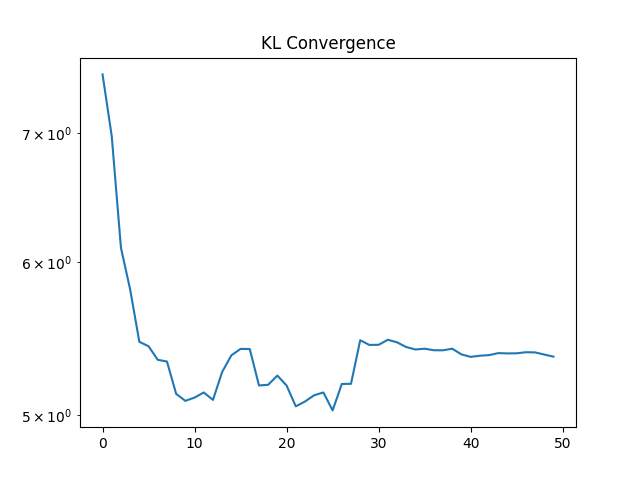
\includegraphics[width=0.7\linewidth]{figures/fig1_kl.png}
\caption{KL convergence under adversarial ratios}
\end{figure}

\input{sections/6_real_world}
\input{sections/7_conclusion}

\bibliographystyle{plain}
\bibliography{bibliography}

\appendix
\input{appendix}

\end{document}

